\subsubsection{Nono periodo (2024/04/07 - 2024/05/02)}
\subsubsubsection{Planning}
\subsubsubsubsection*{Attività pianificate}
Gli obiettivi posti per lo $\textit{sprint}_G$ sono stati i seguenti:
\begin{itemize}
    \item Effettuare un incontro con il proponente fissato in data 10 Aprile in cui mostrare quanto fatto nel $\textit{PoC}_G$;
    \item Effettuare il colloquio con il prof. Cardin per la revisione $\textit{RTB}_G$ in data 12 Aprile per il quale si vuole:
    \begin{itemize}
        \item Preparare le diapositive per il colloquio;
        \item Preparare la lettera di presentazione per la fase $\textit{RTB}_G$.
    \end{itemize}
    \item Per quanto riguarda il $\textit{Piano di Qualifica}_G$ si vuole:
    \begin{itemize}
        \item Individuare le metriche da inserire nella sezione \emph{"Cruscotto di valutazione della qualità"};
        \item Stilare di conseguenza la sezione di \emph{"Modifiche migliorative"};
        \item Aggiornare la sezione \emph{Test di sistema} in base a quanto riportato nell'ultimo aggiornamento dell'Analisi dei Requisiti in particolare riguardo ai requisiti.
    \end{itemize}
    \item Effettuare delle correzioni (eventuali) all'Analisi dei Requisiti fornite dal prof. Cardin in fase di revisione $\textit{RTB}_G$.
    \item Aggiornare $\textit{Norme di Progetto}_G$, inserendo alcune sezioni mancanti come \emph{Validazione}, \emph{repository Proof of Concept} e inserendo come vengono gestite le procedure per alcuni ruoli.
\end{itemize}
\subsubsubsubsection*{Preventivo}
\begin{table}[H]
    \centering
\begin{spreadtab}{{tabular}{|c|c|c|c|c|c|c|c|}}
    \hline
    @\textbf{Membro} & @\textbf{Re} & @\textbf{Amm} & @\textbf{An} & @\textbf{Progr} & @\textbf{Proge} & @\textbf{Ve} & @\textbf{Totale} \\
    \hline
    @ Samuele V.   & 0          & 2.42          & 0         & 0.25          & 0     & 0.55     & sum(b2:g2) \\
    @ Leonardo B.  & 0         & 0          & 1        & 0        & 0     & 2.92    & sum(b3:g3) \\
    @ Riccardo Z.  & 1.5          & 2.5          & 0          & 0.67         & 0     & 0.25  & sum(b4:g4) \\
    @ Davide B.    & 2.5          & 2.5         & 0       & 0       & 0     & 0     & sum(b5:g5) \\
    @ Michele Z.   & 0          & 2.5          & 1.5         & 0          & 0     & 1.67     & sum(b6:g6) \\
    @ Filippo T.   & 0          & 1.83          & 2         & 0.33          & 0     & 0     & sum(b7:g7) \\
    \hline
    @\textbf{Ore totali} & sum(b2:b7) & sum(c2:c7) & sum(d2:d7) & sum(e2:e7) & sum(f2:f7) & sum(g2:g7) &  sum(b8:g8)\\
    \hline
    @\textbf{Costo totale} & 30*b8 & 20*c8 & 25*d8 & 15*e8 & 25*f8 & 15*g8 & sum(b9:g9)\\
    \hline
\end{spreadtab}
    \caption{Preventivo orario ed economico parziale per il nono periodo, in base al ruolo}
    \label{tab:prev_rtb}
    \vspace{5mm}
    \textbf{Legenda:} \textit{Re} = Responsabile, \textit{Amm} = Amministratore, \textit{An} = Analista, \textit{Progr} = Programmatore, \textit{Proge} = Progettista, \textit{Ve} = Verificatore
\end{table}
\subsubsubsection{Review}
\subsubsubsubsection*{Attività svolte}
Le attività svolte in questo periodo sono state le seguenti:
\begin{itemize}
    \item Effettuato un incontro con il proponente per mostrare quanto sviluppato per il $\textit{PoC}_G$ in cui:
    \begin{itemize}
        \item è emerso l'apprezzamento per la $\textit{feature}_G$ di $\textit{ordinazione}_G$ collaborativa;
        \item è emerso che in futuro si debba prendere in considerazione la paginazione per gestire una grande mole di dati in funzionalità quali la ricerca del ristorante;
        \item si è discusso di architetture come Kafka;
        \item si è parlato della possibilità di impostare un progetto implementando un'$\textit{architettura}_G$ a microservizi.
    \end{itemize}
    \item Effettuato il colloquio con il prof. Cardin per la revisione $\textit{RTB}_G$ presentando le relative diapositive, il quale è risultato in un semaforo verde con le relative correzioni da effettuare al documento di Analisi dei Requisiti.
    \item Aggiornato $\textit{Norme di Progetto}_G$ e inserite le sezioni mancanti;
    \item Aggiornato $\textit{Piano di Qualifica}_G$ e inserite le metriche nella sezione riguardante il cruscotto;
    \item Corretto il documento di Analisi dei Requisiti con le indicazioni del prof. Cardin;
    \item Aggiornato il presente documento con i relativi grafici per ogni periodo;
    \item Preparata la lettera di presentazione e decisa la data di consegna del progetto rivista.
\end{itemize}
\subsubsubsubsection*{Consuntivo}
\begin{table}[H]
    \centering
\begin{spreadtab}{{tabular}{|c|c|c|c|c|c|c|c|}}
    \hline
    @\textbf{Membro} & @\textbf{Re} & @\textbf{Amm} & @\textbf{An} & @\textbf{Progr} & @\textbf{Proge} & @\textbf{Ve} & @\textbf{Totale} \\
    \hline
    @ Samuele V.   & 0          & 2.08          & 0         & 0.17          & 0     & 0.58     & sum(b2:g2) \\
    @ Leonardo B.  & 0         & 0          & 1        & 0        & 0     & 2.67    & sum(b3:g3) \\
    @ Riccardo Z.  & 1.17          & 1.5          & 0          & 0.67         & 0     & 0.42   & sum(b4:g4) \\
    @ Davide B.    & 2          & 2         & 0       & 0       & 0     & 0     & sum(b5:g5) \\
    @ Michele Z.   & 0          & 1.5          & 0         & 0          & 0     & 0.83     & sum(b6:g6) \\
    @ Filippo T.   & 0          & 1.33          & 1.75         & 0.33          & 0     & 0     & sum(b7:g7) \\
    \hline
    @\textbf{Ore totali} & sum(b2:b7) & sum(c2:c7) & sum(d2:d7) & sum(e2:e7) & sum(f2:f7) & sum(g2:g7) &  sum(b8:g8)\\
    \hline
    @\textbf{Costo totale} & 30*b8 & 20*c8 & 25*d8 & 15*e8 & 25*f8 & 15*g8 & sum(b9:g9)\\
    \hline
\end{spreadtab}
    \caption{Consuntivo orario ed economico parziale per il nono periodo, in base al ruolo}
    \label{tab:prev_rtb}
    \vspace{5mm}
    \textbf{Legenda:} \textit{Re} = Responsabile, \textit{Amm} = Amministratore, \textit{An} = Analista, \textit{Progr} = Programmatore, \textit{Proge} = Progettista, \textit{Ve} = Verificatore
\end{table}

\begin{figure}[H]
  \centering
  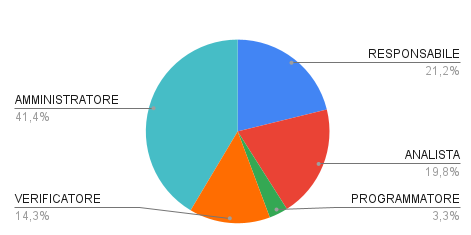
\includegraphics[width=0.6\linewidth]{grafici/9_periodo_torta.png}
  \caption{Ripartizione dei costi per ruolo nel $9^\circ$ periodo}
        \vspace{5mm}
  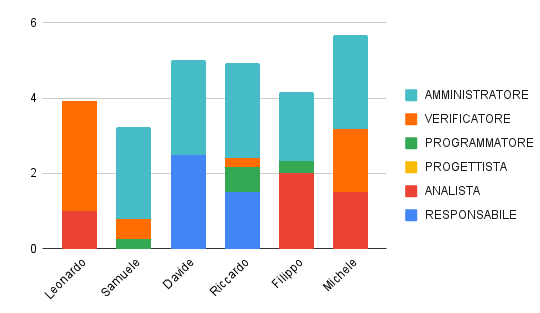
\includegraphics[width=0.7\linewidth]{grafici/9_periodo_istogramma.png}
  \caption{Ore preventivate per ciascuna persona nel $9^\circ$ periodo}
\end{figure}

\subsubsubsection{Retrospective}
La stesura dei documenti si è rilevata più' dispendiosa del previsto e tali documenti sono stati approvati più' tardi rispetto a quanto stabilito all'inizio del periodo. In particolare:
\begin{itemize}
    \item Per l'Analisi dei Requisiti non era chiaro ad alcuni membri del gruppo come poter effettuare le correzioni indicate;
    \item E' emerso che in futuro si dovranno distribuire più' correttamente le attività in base alle disponibilità di ciascun membro.
\end{itemize}